\documentclass[utf-8, 10pt]{article}

\usepackage{ctex}

\usepackage[
    paperwidth=210mm,
    paperheight=297mm,
    top=31.8mm,
    bottom=31.8mm,
    left=25.4mm,
    right=25.4mm,
    footskip=15mm % 通过这里的值来调整页脚与正文内容的垂直距离
]{geometry}

\usepackage{titlesec} % 定义标题样式

% 定义 section 标题格式
\titleformat{\section}[hang]{\heiti\centering\large\bfseries}{\thesection}{1em}{}

% 定义 subsection 标题格式
\titleformat{\subsection}[hang]{\heiti\bfseries}{\textbf{\thesubsection}}{1em}{}

% 定义 subsubsection 标题格式
\titleformat{\subsubsection}[hang]{\kaishu}{\quad\quad\thesubsubsection\,\,}{0em}{}

\usepackage{mdframed}
\mdfsetup{
  linewidth=0.4pt,
  frametitlebackgroundcolor=white, % 或者 transparent
  frametitlefont=\heiti\bfseries,
  frametitleaboveskip=10pt,
  frametitlebelowskip=5pt,
  frametitlealignment=\raggedright % 新增此行
}
\usepackage{fontspec}
% 设置 Menlo 字体
\setmonofont{Menlo}
\usepackage{fancyvrb}
\usepackage{xcolor}
\usepackage{listings}

% \definecolor{string}{HTML}{067D17}
% \definecolor{comment}{HTML}{8C8C8C}
% \definecolor{keyword}{HTML}{0033B3}
% \definecolor{class_field}{HTML}{871094}

\lstset{breaklines}
%这条命令可以让LaTeX自动将长的代码行换行排版
\lstset{extendedchars=false}
%这一条命令可以解决代码跨页时,章节标题,页眉等汉字不显示的问题
\lstset{escapeinside={(*}{*)}}

\lstset{
    basicstyle=\small\ttfamily\heiti,
    numbers=left,
    numberstyle=\scriptsize\fontspec{Menlo}, % 使用 Menlo 字体
    stepnumber=1,
    numbersep=8pt,
    frame=leftline,
    xleftmargin=2em, % 调整代码块的左边界
    framexleftmargin=0pt, % 调整边框的位置
    breaklines=true,
    % postbreak=\mbox{\textcolor{red}{$\hookrightarrow$}\space},
    % keywordstyle=\bfseries\color{keyword},          % keyword style
    % commentstyle=\heiti\color{comment},       % comment style
    % stringstyle=\color[HTML]{067D17},
    showstringspaces=false,
    % string literal style
    % escapeinside={\%*}{*)},            % if you want to add LaTeX within your code
    % morekeywords={}               % if you want to add more keywords to the set
}

\usepackage{fancyhdr} % 用于自定义页眉页脚


% 设置页眉页脚样式
\fancypagestyle{plain}{%
    \fancyhf{} % 清空页眉页脚
    \fancyhead[L]{·\thepage·} % 页眉显示页码, RO表示奇数页右侧, LE表示偶数页左侧
    \fancyhead[R]{马克思主义基本原理}
    \renewcommand{\headrulewidth}{0.4pt} % 设置页眉横线的宽度
    \renewcommand{\footrulewidth}{0pt} % 取消页脚横线
}

\renewcommand{\headrule}{\hrule width\textwidth height\headrulewidth\vskip-\headrulewidth}

% 定义取消页眉的命令
\newcommand{\cancelheader}{%
    \fancyhead{} % 清空页眉
    \renewcommand{\headrulewidth}{0pt} % 取消页眉横线
    \renewcommand{\footrulewidth}{0pt} % 设置页脚横线的宽度
}

\usepackage{caption, subcaption}
\usepackage{longtable, diagbox, booktabs}
\usepackage{float, graphicx}
\usepackage{amsthm, amssymb, amsmath, mathrsfs, mhchem, siunitx, pgfplots}
\usepackage{tikz, circuitikz, tikz-cd, tikz-3dplot}
\usetikzlibrary{decorations.markings, angles, quotes}
\usepackage{tasks, enumitem}
\usepackage{hyperref}
\hypersetup{hidelinks,
    colorlinks = true,
    allcolors = black,
    pdfstartview = Fit,
    breaklinks = true}
\usepackage[toc]{multitoc}
\usepackage{abstract}
\usepackage{extpfeil}
\usepackage{xcolor}

\everymath{\displaystyle}

\begin{document}
\newtheoremstyle{mytheoremstyle}
    {1.5ex}                                         % Space above
    {1.5ex}                                         % Space below
    {}                                              % Font for body
    {}                                              % Indent amount
    {\bfseries}                                     % Font for head
    {}                                              % Punctuation after head
    {0.5em plus 0.2em minus 0.1em}                  % Space after head
    {\thmname{#1}\thmnumber{ #2}.\thmnote{ (#3).}}

\theoremstyle{mytheoremstyle}
\newtheorem{definition}{定义}[section]
\newtheorem{example}{例}[section]
\newtheorem{exercise}{习题}[section]
\newtheorem{code}{程序清单}[section]
\newtheorem*{result}{运行结果}
\newtheorem*{keywords}{关键词}

\newtheoremstyle{my2theoremstyle}
    {1.5ex}                                         % Space above
    {1.5ex}                                         % Space below
    {\kaishu}                                              % Font for body
    {}                                              % Indent amount
    {\bfseries}                                     % Font for head
    {}                                              % Punctuation after head
    {0.5em plus 0.2em minus 0.1em}                  % Space after head
    {\thmname{#1}\thmnumber{ #2}.\thmnote{ (#3).}}

\theoremstyle{my2theoremstyle}
\newtheorem{thm}{定理}[section]
\newtheorem{law}{定律}[section]
\newtheorem{educt}{推论}
\newtheorem{prop}{命题}
\newtheorem{lemma}{引理}
\newtheorem{axiom}{公理}
\newtheorem{property}{性质}

\newtheoremstyle{my4theoremstyle}
    {1.5ex}                                         % Space above
    {1.5ex}                                         % Space below
    {}                                              % Font for body
    {}                                              % Indent amount
    {\bfseries}                                     % Font for head
    {}                                              % Punctuation after head
    {0.5em plus 0.2em minus 0.1em}                  % Space after head
    {\thmname{#1}.}

\theoremstyle{my4theoremstyle} \newtheorem*{sol}{解}

\newtheoremstyle{my3theoremstyle}
    {1.5ex}                                         % Space above
    {1.5ex}                                         % Space below
    {}                                              % Font for body
    {}                                              % Indent amount
    {\kaishu}                                       % Font for head
    {}                                              % Punctuation after head
    {0.5em plus 0.2em minus 0.1em}                  % Space after head
    {\thmname{#1}\thmnumber{ #2}.\thmnote{ (#3).}}

\theoremstyle{my3theoremstyle} \newtheorem*{remark}{注}
\newtheorem*{cmt}{评注}
% \pagestyle{plain}
\title{世界的物质性及发展规律}
\author{钱锋\thanks{电子邮件: strik0r.qf@gmail.com
\newline \indent 西北工业大学软件学院, School of Software, Northwestern Polytechnical University, 西安 710072
}}

\maketitle
\thispagestyle{empty}
% \begin{abstract}
    
%     \begin{keywords}

%     \end{keywords}
% \end{abstract}
{\small \tableofcontents}

\section{世界的多样性与物质统一性}

\subsection{物质及其存在方式}

% \subsection{哲学是系统化、理论化的世界观}

哲学是系统化、理论化的世界观,是对自然知识、社会知识和思维知识的概括和总结,
哲学世界观起源于人类在生活实践中对世界的追问和思考,
是关于宇宙和人生的总体性认识,为人类安身立命提供不可或缺的思想基础。

\begin{figure}[H]
    \centering


\tikzset{every picture/.style={line width=0.75pt}} %set default line width to 0.75pt        

\begin{tikzpicture}[x=0.75pt,y=0.75pt,yscale=-1,xscale=1]
%uncomment if require: \path (0,300); %set diagram left start at 0, and has height of 300

%Straight Lines [id:da06915972307109763] 
\draw    (308,110.5) -- (308,150.5) ;
\draw [shift={(308,153.5)}, rotate = 270] [fill={rgb, 255:red, 0; green, 0; blue, 0 }  ][line width=0.08]  [draw opacity=0] (6.25,-3) -- (0,0) -- (6.25,3) -- cycle    ;

% Text Node
\draw (174,81) node [anchor=north west][inner sep=0.75pt]   [align=left] {世界观:人们对世界的总的看法和根本观点};
% Text Node
\draw (174,166) node [anchor=north west][inner sep=0.75pt]   [align=left] {方法论:人们认识世界和改造世界的根本原则和根本方法};
% Text Node
\draw (319,121) node [anchor=north west][inner sep=0.75pt]   [align=left] {决定};


\end{tikzpicture}
\caption{世界观与方法论}
\end{figure}

\begin{figure}[H]
    \centering
    



    \tikzset{every picture/.style={line width=0.75pt}} %set default line width to 0.75pt        

    \begin{tikzpicture}[x=0.75pt,y=0.75pt,yscale=-1,xscale=1]
    %uncomment if require: \path (0,300); %set diagram left start at 0, and has height of 300
    
    %Shape: Brace [id:dp1198995538704497] 
    \draw   (236,73.5) .. controls (231.33,73.5) and (229,75.83) .. (229,80.5) -- (229,111.25) .. controls (229,117.92) and (226.67,121.25) .. (222,121.25) .. controls (226.67,121.25) and (229,124.58) .. (229,131.25)(229,128.25) -- (229,162) .. controls (229,166.67) and (231.33,169) .. (236,169) ;
    %Shape: Brace [id:dp05903287158077408] 
    \draw   (457,74.5) .. controls (452.33,74.5) and (450,76.83) .. (450,81.5) -- (450,112.25) .. controls (450,118.92) and (447.67,122.25) .. (443,122.25) .. controls (447.67,122.25) and (450,125.58) .. (450,132.25)(450,129.25) -- (450,163) .. controls (450,167.67) and (452.33,170) .. (457,170) ;
    %Straight Lines [id:da8154346896000187] 
    \draw    (175.5,156.5) -- (175.5,196.5) ;
    \draw [shift={(175.5,199.5)}, rotate = 270] [fill={rgb, 255:red, 0; green, 0; blue, 0 }  ][line width=0.08]  [draw opacity=0] (5.36,-2.57) -- (0,0) -- (5.36,2.57) -- cycle    ;
    
    % Text Node
    \draw    (353,108.25) -- (440,108.25) -- (440,136.25) -- (353,136.25) -- cycle  ;
    \draw (396.5,122.25) node   [align=left] {\begin{minipage}[lt]{56.44pt}\setlength\topsep{0pt}
    \begin{center}
    人类活动
    \end{center}
    
    \end{minipage}};
    % Text Node
    \draw    (460,57.75) -- (547,57.75) -- (547,92.75) -- (460,92.75) -- cycle  ;
    \draw (503.5,75.25) node   [align=left] {\begin{minipage}[lt]{56.44pt}\setlength\topsep{0pt}
    \begin{center}
    认识世界
    \end{center}
    
    \end{minipage}};
    % Text Node
    \draw    (461,151.75) -- (548,151.75) -- (548,186.75) -- (461,186.75) -- cycle  ;
    \draw (504.5,169.25) node   [align=left] {\begin{minipage}[lt]{56.44pt}\setlength\topsep{0pt}
    \begin{center}
    改造世界
    \end{center}
    
    \end{minipage}};
    % Text Node
    \draw (187,225.75) node   [align=left] {\begin{minipage}[lt]{72.08pt}\setlength\topsep{0pt}
    具有多样性\\和物质统一性
    \end{minipage}};
    % Text Node
    \draw    (132,94.75) -- (219,94.75) -- (219,149.75) -- (132,149.75) -- cycle  ;
    \draw (175.5,122.25) node   [align=left] {\begin{minipage}[lt]{56.44pt}\setlength\topsep{0pt}
    \begin{center}
    世界上的\\各种现象
    \end{center}
    
    \end{minipage}};
    % Text Node
    \draw    (239,56.75) -- (326,56.75) -- (326,91.75) -- (239,91.75) -- cycle  ;
    \draw (282.5,74.25) node   [align=left] {\begin{minipage}[lt]{56.44pt}\setlength\topsep{0pt}
    \begin{center}
    物质现象
    \end{center}
    
    \end{minipage}};
    % Text Node
    \draw    (239,149.75) -- (326,149.75) -- (326,184.75) -- (239,184.75) -- cycle  ;
    \draw (282.5,167.25) node   [align=left] {\begin{minipage}[lt]{56.44pt}\setlength\topsep{0pt}
    \begin{center}
    精神现象
    \end{center}
    
    \end{minipage}};
    
    
    \end{tikzpicture}
\caption{世界上的万事万物归结起来无非是两大类现象,即物质现象和精神现象;
人类的活动归结起来无非也是两大类,即认识世界和改造世界}
\end{figure}

% \section{哲学及其基本问题}

恩格斯总结和概括了哲学发展,特别是近代哲学发展的历史事实,第一次明确提出:“全部哲学
问题,特别是近代哲学的重大的基本问题,是思维和存在的关系问题。” 哲学基本问题主要包括
两个方面的内容:
\begin{enumerate}[label={$\left.\arabic*\right)$}, itemsep=0pt]
    \item 存在和思维、物质和意识谁为本原的问题,即何者为第一性的问题,
    对这一问题的不同回答,形成了唯物主义和唯心主义两种根本对立的哲学派别。
    \item 存在和思维、物质和意识是否具有同一性的问题,即思维能否正确地反映存在、
    人能否认识或彻底认识世界的问题,
    对这一问题的不同回答,产生了可知论和不可知论的理论分野。
\end{enumerate}
对哲学基本问题的回答是解决其他一切哲学问题的前提和基础。
只有科学解决存在和思维的关系问题,才能正确认识世界的本质和把握世界发展的规律。

\vspace{1em}

哲学的第一个基本问题是,存在和思维、物质和意识谁为本原的问题,即何者为第一性的问题。
对这一问题的不同回答,形成了唯物主义和唯心主义两种根本对立的哲学派别。

% \subsubsection{唯物主义}

凡是主张物质是本原,物质第一性、精神第二性的哲学流派,都属于唯物主义,
唯物主义坚持 “从物到感觉和思想” 的认识路线。唯物主义哲学在其历史发展过程中,
依次表现为三种基本的历史形态,即古代朴素唯物主义、近代机械唯物主义和马克思主义
的辩证唯物主义。
\begin{itemize}[itemsep=0pt]
    \item 古代朴素唯物主义的主要特征是以自然原因去解释自然现象,肯定世界的
    物质本原性和统一性。它的主要缺陷是把某种具体的物质形态看作世界的物质本原和统一的
    物质基础,具有明显的 “猜测” 的性质。
    \item 近代形而上学唯物主义以近代科学对自然现象的实证研究为基础,以新的实证知识和科学方法
    论证世界的物质统一性,摆脱了古代唯物主义的朴素性;近代唯物主义自觉地提出并探讨了思维和存在
    的关系问题,主要研究了认识内容的来源等问题,确认了唯物主义的反映论和可知论原则。

    近代唯物主义的局限性在于:
    \begin{enumerate}[label={${\arabic*}^\circ$}, itemsep=0pt]
        \item 把自然界中各种现象和过程归结为机械运动,用力学规律加以解释;
        \item 用孤立、静止、片面的观点解释世界,是一种形而上学的思维方式;
        \item 唯物主义的不彻底性,即自然观的唯物主义、历史观的唯心主义。
    \end{enumerate}
    \item 马克思、恩格斯创立的辩证唯物主义和历史唯物主义是哲学唯物主义的
    最高形态,它克服了就唯物主义的局限性和不彻底性,实现了唯物论与辩证唯物
    法、唯物主义的自然观与历史观的统一。
\end{itemize}

% \subsubsection{唯心主义}

凡是断言精神对自然界来说是本原,精神第一性、物质第二性的哲学流派,都属于唯心主义,
唯心主义坚持 “从思想和感觉到物” 的认识路线。
在哲学史上,唯心主义哲学有众多流派,归结起来有两种基本形式:一是主观唯心主义,一是客观
唯心主义。
\begin{itemize}[itemsep=0pt]
    \item 主观唯心主义把个人的感觉、心灵、意识、观念夸大为第一性的东西,否认物质世界
    和客观规律不依赖于人的意识而存在。
    \item 客观唯心主义则把某种 “客观精神” 说成是先于病独立于物质世界的存在,并把物质世界
    说成是这种 “客观精神” 的产物、表现或附属品。
\end{itemize}
在对思维与存在、精神与物质的关系的理解和解释中,如果 “把认识的某一特征、某一方面、某一侧面,
片面地、夸大地……发展(膨胀、扩大)为脱离了物质、脱离了自然的、神话了的绝对”,就会
导致唯心主义。

% \subsection{}
哲学的第二个基本问题是,存在和思维、物质和意识是否具有同一性的问题,即思维能否正确地反映存在、人能否认识或彻底认识世界的问题。
依据对思维和存在是否具有同一性、我们的思维能不能认识现实问题的不同回答,可以把哲学区分为
可知论和不可知论。
\begin{itemize}[itemsep=0pt]
    \item 绝大多数哲学学派都属于可知论,但唯物主义和唯心主义的可知论是方向不同的可知论。
    唯物主义的可知论认为人的思维能够正确地反映现实世界,而唯心主义的可知论则用精神的本原性
    来说明思维和存在的统一性的可知论。
    \item 凡是对思维和存在是否具有统一性做出否定回答的哲学理论,都属于不可知论。
\end{itemize}

\subsubsection{哲学的物质范畴}

古代朴素唯物主义用某一种或几种物质作为本原来解释世界,在当时具有合理性和进步性。
但是,把物质等同于具体的物质形态,又有明显的局限性。近代形而上学唯物主义以近代科学为基础,
把物质等同于物质的微观结构层次——原子,虽然使唯物主义对物质概念的理解建立在自然科学发现
的基础上,却不能正确理解哲学的物质概念与自然科学的物质概念之间共性与个性的关系,
更无法将唯物主义贯彻到历史领域中,无法说明社会运动的物质性。

% 哲学上关于 “物质” 的概念有许多种提法(要注意把它们与自然科学关于具体的物质形态和物质结构的
% 概念区分开来),我们要重点学习的是恩格斯和列宁的关于物质概念的提法:
马克思、恩格斯批判了旧唯物主义对物质世界的直观、消极、机械的理解,强调要用辩证的观点把握世界,
特别是要从实践出发去把握现实世界,从自然存在和社会存在的统一中去把握世界的物质性。
马克思主义的 “物质” 范畴是一个高度抽象的哲学概念,是对世界上客观存在的各种事物
共同本质的概括。
\begin{itemize}[itemsep=0pt]
    \item \textbf{恩格斯关于物质概念的提法}:“物、物质无非就是各种物的总和,而这个概念就是从
    这一总和中抽象出来的”。
    % 这就是说,物质这个名词是一种简称,“我们就用这种简称把感官可感知的
    % 许多不同的事物依照其共同的属性概括起来”。
    % 这个提法明确指出了\textbf{哲学物质概念与自然科学关于具体的物质形态和物质结构的
    % 概念之间的共性与个性、普遍与特殊、具体和抽象的关系}。
    % \begin{remark}
    %     哲学物质概念与自然科学关于具体的物质形态和物质结构的概念之间不是 “整体和部分” 的关系!
    % \end{remark}
    \item \textbf{列宁关于物质概念的提法}:物质是标志客观实在的哲学范畴,这种客观实在
    \begin{enumerate}[label=\textup{\arabic*}${}^\circ$, itemsep=0pt]
        \item 是人通过感觉感知的;
        \item \textbf{是不依赖于我们的感觉而存在的};
        \item 是为我们的感觉所复写、摄影、反映的。
    \end{enumerate}

    % 定义方式:\textbf{列宁是从物质与意识的关系上来把握物质的}。

    % 物质范畴是对物质世界多样性和统一性所作的最高的哲学概括,\textbf{物质的共同特征、唯一特征是客观实在性},
    % 它存在于人类的意识之外,为人类的意识所反映。
    % \begin{remark}
    %     判断一个东西是否是物质的标准,就是它是否 “不依赖于我们的感觉而存在”。
    % \end{remark}
\end{itemize}
这一定义表明,物质是不依赖于人类的意识而存在,并能为人类的意识所反映的客观实在。
这种客观实在性,是从自然存在和社会存在中抽象出的共同特性。

\subsubsection{物质的存在方式}

物质的根本属性和存在方式是很么?运动着的物质的基本存在形式又是什么?

\begin{figure}[H]
    \centering


    \tikzset{every picture/.style={line width=0.75pt}} %set default line width to 0.75pt        

    \begin{tikzpicture}[x=0.75pt,y=0.75pt,yscale=-1,xscale=1]
    %uncomment if require: \path (0,300); %set diagram left start at 0, and has height of 300
    
    %Shape: Brace [id:dp5396784354798981] 
    \draw   (98,108) .. controls (93.33,108) and (91,110.33) .. (91,115) -- (91,150.25) .. controls (91,156.92) and (88.67,160.25) .. (84,160.25) .. controls (88.67,160.25) and (91,163.58) .. (91,170.25)(91,167.25) -- (91,205.5) .. controls (91,210.17) and (93.33,212.5) .. (98,212.5) ;
    %Straight Lines [id:da8349474099648175] 
    \draw    (209,109) -- (283,109) ;
    \draw [shift={(286,109)}, rotate = 180] [fill={rgb, 255:red, 0; green, 0; blue, 0 }  ][line width=0.08]  [draw opacity=0] (5.36,-2.57) -- (0,0) -- (5.36,2.57) -- cycle    ;
    %Straight Lines [id:da4818301777895936] 
    \draw    (221,213) -- (283,213) ;
    \draw [shift={(286,213)}, rotate = 180] [fill={rgb, 255:red, 0; green, 0; blue, 0 }  ][line width=0.08]  [draw opacity=0] (5.36,-2.57) -- (0,0) -- (5.36,2.57) -- cycle    ;
    %Straight Lines [id:da614178840929528] 
    \draw    (331,109) -- (402,109) ;
    \draw [shift={(405,109)}, rotate = 180] [fill={rgb, 255:red, 0; green, 0; blue, 0 }  ][line width=0.08]  [draw opacity=0] (5.36,-2.57) -- (0,0) -- (5.36,2.57) -- cycle    ;
    \draw [shift={(328,109)}, rotate = 0] [fill={rgb, 255:red, 0; green, 0; blue, 0 }  ][line width=0.08]  [draw opacity=0] (5.36,-2.57) -- (0,0) -- (5.36,2.57) -- cycle    ;
    %Straight Lines [id:da06975531545558333] 
    \draw  [dash pattern={on 4.5pt off 4.5pt}]  (426,56.5) -- (426,91.5) ;
    %Straight Lines [id:da40660857551724394] 
    \draw  [dash pattern={on 4.5pt off 4.5pt}]  (307,56.5) -- (307,91.5) ;
    %Shape: Brace [id:dp6981372480973064] 
    \draw   (389,173) .. controls (384.33,173) and (382,175.33) .. (382,180) -- (382,202.75) .. controls (382,209.42) and (379.67,212.75) .. (375,212.75) .. controls (379.67,212.75) and (382,216.08) .. (382,222.75)(382,219.75) -- (382,245.5) .. controls (382,250.17) and (384.33,252.5) .. (389,252.5) ;
    %Straight Lines [id:da4140572639136836] 
    \draw  [dash pattern={on 4.5pt off 4.5pt}]  (540,184.38) -- (507,184.38) ;
    %Straight Lines [id:da21808382125862624] 
    \draw  [dash pattern={on 4.5pt off 4.5pt}]  (540,260.38) -- (507,260.38) ;
    %Straight Lines [id:da35114719364911073] 
    \draw    (307,128.5) -- (307,192.5) ;
    \draw [shift={(307,195.5)}, rotate = 270] [fill={rgb, 255:red, 0; green, 0; blue, 0 }  ][line width=0.08]  [draw opacity=0] (5.36,-2.57) -- (0,0) -- (5.36,2.57) -- cycle    ;
    \draw [shift={(307,125.5)}, rotate = 90] [fill={rgb, 255:red, 0; green, 0; blue, 0 }  ][line width=0.08]  [draw opacity=0] (5.36,-2.57) -- (0,0) -- (5.36,2.57) -- cycle    ;
    %Shape: Rectangle [id:dp06362495612482066] 
    \draw   (101,82.5) -- (150,82.5) -- (150,112.5) -- (101,112.5) -- cycle ;
    %Curve Lines [id:da6459325889321588] 
    \draw    (126.03,78.62) .. controls (137.75,18.94) and (300.51,61.91) .. (306.83,94.98) ;
    \draw [shift={(307,97.5)}, rotate = 273.37] [fill={rgb, 255:red, 0; green, 0; blue, 0 }  ][line width=0.08]  [draw opacity=0] (5.36,-2.57) -- (0,0) -- (5.36,2.57) -- cycle    ;
    \draw [shift={(125.5,82.5)}, rotate = 274.69] [fill={rgb, 255:red, 0; green, 0; blue, 0 }  ][line width=0.08]  [draw opacity=0] (5.36,-2.57) -- (0,0) -- (5.36,2.57) -- cycle    ;
    
    % Text Node
    \draw (157,109) node   [align=left] {\begin{minipage}[lt]{68pt}\setlength\topsep{0pt}
    物质的根本属性或存在方式
    \end{minipage}};
    % Text Node
    \draw (307,109) node   [align=left] {\begin{minipage}[lt]{25.84pt}\setlength\topsep{0pt}
    \begin{center}
    运动
    \end{center}
    
    \end{minipage}};
    % Text Node
    \draw (163,213) node   [align=left] {\begin{minipage}[lt]{76.16pt}\setlength\topsep{0pt}
    运动着的物质的基本存在形式
    \end{minipage}};
    % Text Node
    \draw (329.5,213) node   [align=left] {\begin{minipage}[lt]{56.44pt}\setlength\topsep{0pt}
    时间与空间
    \end{minipage}};
    % Text Node
    \draw (426,109) node   [align=left] {\begin{minipage}[lt]{25.84pt}\setlength\topsep{0pt}
    \begin{center}
    静止
    \end{center}
    
    \end{minipage}};
    % Text Node
    \draw (366.5,93) node  [font=\small] [align=left] {\begin{minipage}[lt]{51pt}\setlength\topsep{0pt}
    \begin{center}
    对立统一
    \end{center}
    
    \end{minipage}};
    % Text Node
    \draw (307,39) node   [align=left] {\begin{minipage}[lt]{36.72pt}\setlength\topsep{0pt}
    \begin{center}
    绝对的
    \end{center}
    
    \end{minipage}};
    % Text Node
    \draw (426,39) node   [align=left] {\begin{minipage}[lt]{36.72pt}\setlength\topsep{0pt}
    \begin{center}
    相对的
    \end{center}
    
    \end{minipage}};
    % Text Node
    \draw (452.5,184.38) node   [align=left] {\begin{minipage}[lt]{74.12pt}\setlength\topsep{0pt}
    物质运动的持续性、顺序性
    \end{minipage}};
    % Text Node
    \draw (451.5,260.38) node   [align=left] {\begin{minipage}[lt]{72.76pt}\setlength\topsep{0pt}
    物质运动的广延性、伸张性
    \end{minipage}};
    % Text Node
    \draw (569,260.38) node   [align=left] {\begin{minipage}[lt]{36.72pt}\setlength\topsep{0pt}
    \begin{center}
    三维的
    \end{center}
    
    \end{minipage}};
    % Text Node
    \draw (569,186) node   [align=left] {\begin{minipage}[lt]{36.72pt}\setlength\topsep{0pt}
    \begin{center}
    一维的
    \end{center}
    
    \end{minipage}};
    % Text Node
    \draw (267.5,164) node  [font=\small] [align=left] {\begin{minipage}[lt]{51pt}\setlength\topsep{0pt}
    \begin{center}
    不可分割
    \end{center}
    
    \end{minipage}};
    % Text Node
    \draw (199.5,41) node  [font=\small] [align=left] {\begin{minipage}[lt]{51pt}\setlength\topsep{0pt}
    \begin{center}
    不可分割
    \end{center}
    
    \end{minipage}};
    
    
    \end{tikzpicture}
\caption{物质、运动、时间、空间}
\end{figure}

首先,
物质的根本属性是运动。恩格斯关于运动概念的提法是:“运动,就它被理解为物质的存在方式、
物质的固有属性这一最一般的意义来说,涵盖宇宙中发生的一切变化和过程,
从单纯的位置变动直到思维”。
这就是说,\textbf{运动是标志一切事物和现象的变化及其过程的哲学范畴}。
从这一运动概念的提法立即得到:
\begin{enumerate}[label={${\arabic*}^\circ$}, itemsep=0pt]
    \item \textbf{运动是物质的存在方式、根本属性和固有属性}。
    \item 马克思主义的运动概念比物理学(尤其是运动学与动力学)中运动的
    概念更加广泛,物体的机械运动、受力运动、定轴转动、机械振动与电磁振荡
    是运动,化学反应、生物化学反应也是运动,人的思维过程也是运动。
\end{enumerate}
\textbf{物质和运动是不可分割的},
运动是物质的运动,物质是运动着的物质,离开物质的运动和离开运动的物质都是不存在的\footnote{
    徐涛老师的政治强化课中对于 “不可分割” 的关系做了一个很有意思的归纳和概括:
    所谓 $A$ 与 $B$ 不可分割,即 $A$ 是 $B$ 的 $A$, $B$ 是 $A$ 的 $B$,
    离开了 $A$ 的 $B$ 与离开了 $B$ 的 $A$ 都是不存在的。
}。

% 脱离物质谈运动,将导致唯心主义;脱离运动谈物质,将导致形而上学。


% \subsection{运动和静止}

其次,\textbf{物质世界的运动是绝对的,而物质在运动过程中又有某种相对的静止}。
相对静止是物质运动在一定条件下的稳定状态,具体包括两种状态:
\begin{itemize}[itemsep=0pt]
    \item 空间相对位置暂时不变;
    \item 根本性质暂时不变。
\end{itemize}
无条件的绝对运动和有条件的相对静止构成了对立统一\footnote{
    徐涛老师的政治强化课中对于对立统一关系也做了一个很有意思的归纳和概括:
    $A$ 与 $B$ 对立统一,即 $A$ 与 $B$ 相互区别,同时 $A$ 与 $B$ 相互联系。
    我们所要做的,就是基于这个框架,具体阐述这对概念的对立性和统一性是怎么具体体现的,
    这就是说,具体解释它们怎么相互区别,又怎么相互联系。
}的关系。
运动的绝对性体现了物质运动的变动性、无条件性,静止的相对性则体现了物质运动
的稳定性、条件性(运动和静止对立性的体现)。
运动和静止相互依赖、相互渗透、相互包含,\textbf{“动中有静、静中有动”}(运动和静止统一性的体现)。
% \begin{itemize}[itemsep=0pt]
%     \item \textbf{静止的概念}:
%     \item \textbf{运动和静止的关系}:对立统一。
%     \begin{remark}
%         
%     \end{remark}
%     \begin{itemize}[itemsep=0pt]
%         \item \textbf{运动和静止的相互区别}:\textbf{运动的绝对性体现了物质运动的变动性、无条件性;静止的
%         相对性体现了物质运动的稳定性、有条件性}。
%         \item \textbf{运动和静止的相互联系}:}。
%     \end{itemize}
%     \item 两种错误的观点:夸大静止、否定运动,将导致形而上学;夸大运动、否定静止,将导致诡辩论。
% \end{itemize}

\begin{example}
    赫拉克利特认为 “人不能两次踏进同一条河流”,但他的学生反驳说 “人一次也不能
    踏进同一条河流”。下列对这两种观点的理解正确的有 \underline{\qquad \qquad \qquad}。
    \begin{tasks}[label={\Alph*.}](2)
        \task 前者是辩证法的观点
        \task 后者是相对主义诡辩论
        \task 前者肯定相对静止
        \task 后者否定绝对运动
    \end{tasks}
    \begin{cmt}
        “人不能两次踏进同一条河流” 体现的思想是物质是运动的, 运动是物质的
        根本属性和存在方式,物质和运动是不可分割的。世界上的一切事物都处在运动变化
        之中,这是辩证唯物主义的思想。辩证唯物主义在承认运动是绝对的同时,还承认
        相对静止的存在。而 “人一次也不能踏进同一条河流” 的思想过分地夸大了运动,
        否定相对静止的存在,陷入了相对主义诡辩论当中。因此本题选择 ABC。
    \end{cmt}
\end{example}

第三,\textbf{时间和空间是运动着的物质的基本存在形式}。时间是指物质运动的
持续性、顺序性,特点是一维性,即时间的流逝一去不复返。空间是指物质运动的广
延性、伸张性,特点是三维性,即空间具有长、宽、高三方面的规定性。
\textbf{物质运动与时空是不可分割的},物质运动总是在一定的时间和空间中
进行的,没有离开物质运动的 “纯粹” 空间和时间,也没有离开时间和空间
的物质运动。

% \subsubsection{物质世界的二重化}

\subsection{物质与意识的辩证关系}

人的意识是物质世界长期发展的产物,是社会实践的产物,物质与意识的关系是辩证统一的。

\subsubsection{物质决定意识}

意识是人脑的机能和属性,是客观世界的主观映象。物质对意识的决定作用表现在意识的起源
和本质上。首先,从意识的起源来看:
\begin{itemize}[itemsep=0pt]
    \item 意识是自然界长期发展的产物。它的形成和发展经历了三个阶段:
    \begin{enumerate}[label={$\left.\arabic*\right)$}, itemsep=0pt]
        \item 从一切物质所具有的反应特性到低等生物的刺激感应性;
        \item 再到高等动物的感觉和心理;
        \item 最终发展为人类的意识。
    \end{enumerate}
    \item 意识是社会历史发展的产物:
    \begin{enumerate}[label={$\left.\arabic*\right)$}, itemsep=0pt]
        \item 社会实践,特别是劳动,在意识的产生和发展中起着决定性的作用。
        劳动为意识的产生和发展提供了客观需要和可能。
        \item 在人们的劳动和交往中形成的语言促进了意识的发展。
    \end{enumerate}
\end{itemize}
其次,从意识的本质来看,\textbf{意识是} \textbf{人脑}这样一种特殊物质
\textbf{的机能和属性},是客观世界的主观映象。意识在内容上是客观的,
在形式上是主观的,是客观内容和主观形式的统一。
意识是物质的产物,但又不是物质本身。

\begin{figure}[H]
    \centering
    

\tikzset{every picture/.style={line width=0.75pt}} %set default line width to 0.75pt        

\begin{tikzpicture}[x=0.75pt,y=0.75pt,yscale=-1,xscale=1]
%uncomment if require: \path (0,300); %set diagram left start at 0, and has height of 300

%Straight Lines [id:da06405785871650937] 
\draw    (264,86.5) -- (235.23,112.49) ;
\draw [shift={(233,114.5)}, rotate = 317.91] [fill={rgb, 255:red, 0; green, 0; blue, 0 }  ][line width=0.08]  [draw opacity=0] (5.36,-2.57) -- (0,0) -- (5.36,2.57) -- cycle    ;
%Straight Lines [id:da9397832976665516] 
\draw    (292,132.5) -- (249,132.5) ;
\draw [shift={(246,132.5)}, rotate = 360] [fill={rgb, 255:red, 0; green, 0; blue, 0 }  ][line width=0.08]  [draw opacity=0] (5.36,-2.57) -- (0,0) -- (5.36,2.57) -- cycle    ;
%Straight Lines [id:da746063512086695] 
\draw    (247,173.5) -- (230.85,152.86) ;
\draw [shift={(229,150.5)}, rotate = 51.95] [fill={rgb, 255:red, 0; green, 0; blue, 0 }  ][line width=0.08]  [draw opacity=0] (5.36,-2.57) -- (0,0) -- (5.36,2.57) -- cycle    ;
%Straight Lines [id:da9369887579003064] 
\draw  [dash pattern={on 4.5pt off 4.5pt}]  (316,77.5) -- (353,77.5) ;
%Straight Lines [id:da5150765964716902] 
\draw  [dash pattern={on 4.5pt off 4.5pt}]  (343,132.5) -- (380,132.5) ;
%Straight Lines [id:da9741770345940048] 
\draw  [dash pattern={on 4.5pt off 4.5pt}]  (341,201) -- (378,201) ;

% Text Node
\draw    (201.5, 129.25) circle [x radius= 33.23, y radius= 20.51]   ;
\draw (201.5,129.25) node   [align=left] {\begin{minipage}[lt]{31.96pt}\setlength\topsep{0pt}
\begin{center}
意识
\end{center}

\end{minipage}};
% Text Node
\draw (268,69) node [anchor=north west][inner sep=0.75pt]   [align=left] {劳动};
% Text Node
\draw (298,124) node [anchor=north west][inner sep=0.75pt]   [align=left] {语言};
% Text Node
\draw (251,182) node [anchor=north west][inner sep=0.75pt]   [align=left] {其他社会历\\史发展因素};
% Text Node
\draw (368,69) node [anchor=north west][inner sep=0.75pt]   [align=left] {决定性因素};
% Text Node
\draw (399,124) node [anchor=north west][inner sep=0.75pt]   [align=left] {促进作用};
% Text Node
\draw (396,192.5) node [anchor=north west][inner sep=0.75pt]   [align=left] {促进作用};


\end{tikzpicture}
\caption{意识是社会历史发展的产物}
\end{figure}

\begin{example}
    (多选)
    凤凰是中国古代传说中的鸟中之王,其雄性叫 “凤”,雌性叫 “凰”,
    总称为 “凤” 或者 “凤凰”。根据《雨雅·释鸟》所记载,凤凰的形体为
    “鸡头、蛇颈、燕颔、龟背、五彩色,高六尺许”。由此可见,
    意识\footnote{
        在徐涛老师的优题库习题集\cite{优题库}中,本题最终的设问是 “人们头脑中的凤凰观念是……”,
        但我本人觉得这个设问配合答案其实并不合理——人们头脑中的凤凰观念是人类意识的一个
        具体的实例,意识包含这一观念但是却比这一观念更加广泛,因此我在这里把最终的
        设问换成了意识是什么。
    }是 \underline{\qquad \qquad \qquad}。
    \begin{tasks}[label={\Alph*.}](2)
        \task 客观世界的主观映象
        \task 人脑对客观世界的创造性反映
        \task 人脑中特有的物质
        \task 人脑的机能和属性
    \end{tasks}
    \begin{cmt}
        意识是客观世界的主观映象,是人脑对客观世界的创造性反映,
        是人脑的机能和属性。因此本题选择 ABD。
        这里需要注意的是,类似 “意识是人脑的分泌物”、“意识是人脑中特有的物质”
        的观点是庸俗唯物主义的观点,混淆了意识与物质的概念。
    \end{cmt}
\end{example}

\subsubsection{意识对物质具有反作用}

物质决定意识,意识对物质具有反作用,这种反作用就是意识的能动作用。这就是说,
\textbf{物质决定意识,但意识能动地反作用于物质。}
意识的能动作用主要表现在:
\begin{figure}[H]
    \centering

\tikzset{every picture/.style={line width=0.75pt}} %set default line width to 0.75pt        

\begin{tikzpicture}[x=0.75pt,y=0.75pt,yscale=-1,xscale=1]
%uncomment if require: \path (0,300); %set diagram left start at 0, and has height of 300

%Shape: Brace [id:dp6717037653773108] 
\draw   (201,79.5) .. controls (196.33,79.5) and (194,81.83) .. (194,86.5) -- (194,124.75) .. controls (194,131.42) and (191.67,134.75) .. (187,134.75) .. controls (191.67,134.75) and (194,138.08) .. (194,144.75)(194,141.75) -- (194,183) .. controls (194,187.67) and (196.33,190) .. (201,190) ;
%Straight Lines [id:da1265384458399238] 
\draw  [dash pattern={on 4.5pt off 4.5pt}]  (381,80.5) -- (418,80.5) ;
%Shape: Brace [id:dp8303029500623369] 
\draw   (362,156.5) .. controls (366.67,156.5) and (369,154.17) .. (369,149.5) -- (369,140.25) .. controls (369,133.58) and (371.33,130.25) .. (376,130.25) .. controls (371.33,130.25) and (369,126.92) .. (369,120.25)(369,123.25) -- (369,111) .. controls (369,106.33) and (366.67,104) .. (362,104) ;
%Straight Lines [id:da5154900684029353] 
\draw  [dash pattern={on 4.5pt off 4.5pt}]  (381,130.5) -- (418,130.5) ;

% Text Node
\draw (152,136) node   [align=left] {\begin{minipage}[lt]{51.68pt}\setlength\topsep{0pt}
意识的能动作用
\end{minipage}};
% Text Node
\draw (214,72) node [anchor=north west][inner sep=0.75pt]   [align=left] {意识的目的性和计划性};
% Text Node
\draw (422,72) node [anchor=north west][inner sep=0.75pt]   [align=left] {主体的选择性};
% Text Node
\draw (214,105) node [anchor=north west][inner sep=0.75pt]   [align=left] {意识的创造性};
% Text Node
\draw (214,137) node [anchor=north west][inner sep=0.75pt]   [align=left] {意识对实践的指导性};
% Text Node
\draw (422,122) node [anchor=north west][inner sep=0.75pt]   [align=left] {实践的创造性};
% Text Node
\draw (214,174) node [anchor=north west][inner sep=0.75pt]   [align=left] {调控行为和生理活动};


\end{tikzpicture}
    \caption{意识的能动作用}
\end{figure}
\begin{enumerate}[label={${\arabic*}^\circ$}, itemsep=0pt]
    \item \textbf{意识具有目的性和计划性}。人在认识客观世界、尊重客观规律的同时,
    还总是根据一定的目的和要求去确定反映什么、不反映什么,以及怎样反映,
    从而表现出主体的选择性。
    \item \textbf{意识具有创造性}:人的意识不仅采取感觉、直觉、表象等形式,
    反映事物的外部现象,而且运用概念、判断、推理等形式,对感性材料进行加工制作
    和选择建构,在思维中构造一个现实中所没有的观念世界。
    \begin{figure}[H]
        \centering


\tikzset{every picture/.style={line width=0.75pt}} %set default line width to 0.75pt        

\begin{tikzpicture}[x=0.75pt,y=0.75pt,yscale=-1,xscale=1]
%uncomment if require: \path (0,300); %set diagram left start at 0, and has height of 300

%Shape: Rectangle [id:dp9192327536336478] 
\draw   (221,41.5) -- (467,41.5) -- (467,133) -- (221,133) -- cycle ;
%Shape: Rectangle [id:dp77288325526019] 
\draw   (290,45.5) -- (460,45.5) -- (460,128) -- (290,128) -- cycle ;
%Shape: Rectangle [id:dp19515254732615261] 
\draw   (221,155.5) -- (467,155.5) -- (467,247) -- (221,247) -- cycle ;
%Shape: Rectangle [id:dp8803354966010318] 
\draw   (291,161.5) -- (461,161.5) -- (461,244) -- (291,244) -- cycle ;
%Curve Lines [id:da5441281578657254] 
\draw    (291,85.5) .. controls (251.8,108.04) and (254.86,178.6) .. (287.94,201.18) ;
\draw [shift={(290,202.5)}, rotate = 210.96] [fill={rgb, 255:red, 0; green, 0; blue, 0 }  ][line width=0.08]  [draw opacity=0] (8.93,-4.29) -- (0,0) -- (8.93,4.29) -- cycle    ;
%Straight Lines [id:da7144092628062131] 
\draw    (212,233) -- (176,233) ;
\draw [shift={(173,233)}, rotate = 360] [fill={rgb, 255:red, 0; green, 0; blue, 0 }  ][line width=0.08]  [draw opacity=0] (5.36,-2.57) -- (0,0) -- (5.36,2.57) -- cycle    ;

% Text Node
\draw (222,114) node [anchor=north west][inner sep=0.75pt]   [align=left] {客观世界};
% Text Node
\draw    (390, 67.5) circle [x radius= 24.04, y radius= 14.85]   ;
\draw (374,59) node [anchor=north west][inner sep=0.75pt]   [align=left] {感觉};
% Text Node
\draw    (426, 104.5) circle [x radius= 24.04, y radius= 14.85]   ;
\draw (410,96) node [anchor=north west][inner sep=0.75pt]   [align=left] {直觉};
% Text Node
\draw    (359, 105.5) circle [x radius= 24.04, y radius= 14.85]   ;
\draw (343,97) node [anchor=north west][inner sep=0.75pt]   [align=left] {表象};
% Text Node
\draw (292,48.5) node [anchor=north west][inner sep=0.75pt]   [align=left] {感性材料};
% Text Node
\draw (224,223) node [anchor=north west][inner sep=0.75pt]   [align=left] {思维};
% Text Node
\draw (293,164.5) node [anchor=north west][inner sep=0.75pt]   [align=left] {观念世界};
% Text Node
\draw (263,137) node [anchor=north west][inner sep=0.75pt]   [align=left] {选择建构};
% Text Node
\draw    (391, 182.5) circle [x radius= 24.04, y radius= 14.85]   ;
\draw (375,174) node [anchor=north west][inner sep=0.75pt]   [align=left] {概念};
% Text Node
\draw    (427, 219.5) circle [x radius= 24.04, y radius= 14.85]   ;
\draw (411,211) node [anchor=north west][inner sep=0.75pt]   [align=left] {推理};
% Text Node
\draw    (360, 220.5) circle [x radius= 24.04, y radius= 14.85]   ;
\draw (344,212) node [anchor=north west][inner sep=0.75pt]   [align=left] {判断};
% Text Node
\draw (121,227) node   [align=left] {\begin{minipage}[lt]{68pt}\setlength\topsep{0pt}
是客观世界的主观映象
\end{minipage}};


\end{tikzpicture}
        \caption{意识具有创造性}
    \end{figure}
    \item \textbf{意识具有指导实践改造客观世界的作用}:意识的能动作用
    不限于从实践中形成一定的思想、形成活动的目的、计划、方法等观念的东西,
    更重要的在于以这些观念的东西作为指导,通过实践使之一步步变成客观现实。
    改变世界或创造世界不仅意味着强化客观世界的变化过程,而且意味着创造出
    世界上原来所没有的东西,即没有人的参与永远也不可能出现的东西。
    \item \textbf{意识具有调控人的行为和生理活动的作用}。现代科学和医学实验
    证明,意识、心理因素能够对人的行为选择和健康状况产生重要影响。
\end{enumerate}

\begin{example}
    马克思说,人在 “劳动过程结束时得到的结果,在这个过程开始时就已经在劳动
    者的表象中存在着,即已经观念地存在着”。这说明意识具有目的性和计划性,
    人的整个实践过程,就是围绕意识活动所构建的目标和蓝图来进行的。
\end{example}

\begin{example}
    列宁说:“世界不会满足人,人决心以自己的行动来改变世界”。这说明了
    意识具有指导实践改造客观世界的作用。
\end{example}

\begin{example}
    物质对意识的决定作用表现在意识的起源、本质和作用上。从意识的起源来看,意识
    既是自然界长期发展的产物,也是社会历史发展的产物。下列表述正确的有 \underline{\qquad \qquad \qquad}。
    \begin{tasks}[label={\Alph*.}](1)
        \task 劳动在意识的产生与发展中起着决定性的作用
        \task 劳动为意识的产生和发展提供了客观需要和可能
        \task 劳动使人在改造世界时充满了创造性
        \task 人们在劳动过程中形成的语言促进了意识的发展
    \end{tasks}
    \begin{cmt}
        劳动作为人的实践活动,在人的意识的产生与发展中起着决定性的作用,
        劳动为意识的产生和发展提供了客观需要和可能,同时劳动也使得人脑变得更加复杂,
        为意识的产生提供了条件。人们头脑当中的意识需要借助语言来表达,所以,
        人们在劳动和交往过程中形成的语言也促进了意识的发展。
        因此本题选择 ABC,需要注意的是,意识具有主观能动性,所以
        意识是有创造性的,但是这与劳动本身并没有关系,是意识的创造性
        使得人类改造世界的劳动充满了创造性。
        \begin{figure}[H]
            \centering


\tikzset{every picture/.style={line width=0.75pt}} %set default line width to 0.75pt        

\begin{tikzpicture}[x=0.75pt,y=0.75pt,yscale=-1,xscale=1]
%uncomment if require: \path (0,300); %set diagram left start at 0, and has height of 300

%Shape: Brace [id:dp06824378325166625] 
\draw   (286,194.5) .. controls (290.67,194.5) and (293,192.17) .. (293,187.5) -- (293,157.75) .. controls (293,151.08) and (295.33,147.75) .. (300,147.75) .. controls (295.33,147.75) and (293,144.42) .. (293,137.75)(293,140.75) -- (293,108) .. controls (293,103.33) and (290.67,101) .. (286,101) ;
%Straight Lines [id:da5392340952646961] 
\draw    (310,147) -- (359,147) ;
\draw [shift={(362,147)}, rotate = 180] [fill={rgb, 255:red, 0; green, 0; blue, 0 }  ][line width=0.08]  [draw opacity=0] (5.36,-2.57) -- (0,0) -- (5.36,2.57) -- cycle    ;

% Text Node
\draw (205,118) node   [align=left] {\begin{minipage}[lt]{110.16pt}\setlength\topsep{0pt}
意识具有指导实践改造客观世界的作用
\end{minipage}};
% Text Node
\draw (225,191.75) node   [align=left] {\begin{minipage}[lt]{80.24pt}\setlength\topsep{0pt}
意识具有创造性
\end{minipage}};
% Text Node
\draw (429,148) node   [align=left] {\begin{minipage}[lt]{76.16pt}\setlength\topsep{0pt}
人类的实践是充满创造性的
\end{minipage}};
% Text Node
\draw (306,129) node [anchor=north west][inner sep=0.75pt]   [align=left] {{\small 因果关系}};


\end{tikzpicture}
\caption{人类的实践是充满创造性的}
        \end{figure}
    \end{cmt}
\end{example}



\subsubsection{主观能动性与客观规律性的辩证统一}

正确认识和把握物质与意识的辩证关系,还需要处理好主观能动性和客观规律性
的关系。
尊重客观规律是正确发挥主观能动性的前提,只有充分发挥主观能动性,才能
正确认识和利用客观规律。

\begin{example}
    (多选)
    科学家在海边考察,发现一只小海龟从沙滩上的一个洞穴中探出头来四处张望,
    这时一直在空中盘旋的海鸟发现了它,便冲了下来,小海龟急忙掉头往回爬。
    科学家见状,顿生恻隐之心,决定帮小海龟一把,把它放到海里去。正当科学家为自己的
    “义举” 沾沾自喜时,始料不及的事情发生了。洞穴里的其他小海龟见爬出去的那只小海龟
    没有回来,以为外面是安全的,纷纷往外爬,这立即引来了一大群海鸟,它们不断冲下来,
    享用者丰盛的美餐。实际上,第一支爬出来的海龟是探路的哨兵,一旦有危险就回去报信。
    科学家出于好心帮了这只小海龟,却害惨了整窝海龟。这个故事给我们的启示有 \underline{\qquad \qquad \qquad}。
    \begin{tasks}[label={\Alph*.}](1)
        \task 认识和把握规律是发挥主观能动性的前提
        \task 一切规律发挥作用的过程都是自发的
        \task 人的活动一定受规律的限制
        \task 实践是客观规律性与主观能动性统一的基础
    \end{tasks}
    \begin{cmt}
        尊重客观规律是正确发挥主观能动性的前提,规律是客观的,不以人的意志为转移,
        只要规律存在就一定会制约人的活动。因此本题选择 ACD,需要注意的是,
        客观规律分为自然规律和社会历史规律,
        自然规律发挥作用是自发的,不以人的意志为转移,但社会历史规律发挥作用必须要通过人
        的有意识、有目的的实践活动才能完成,并不是自发的。
    \end{cmt}
\end{example}

\begin{example}
    (多选)
    “揠苗助长” 却事与愿违,“庖丁解牛” 则事半功倍。这两则结果不同的寓言故事共同说明
    的哲学道理有 \underline{\qquad \qquad \qquad}。
    \begin{tasks}[label={\Alph*.}](2)
        \task 不同的人对同一事物有不同的反映
        \task 人具有主观能动性,可以改变和利用规律
        \task 发挥主观能动性必须以尊重规律为前提
        \task 物质决定意识,意识对物质具有巨大的反作用
    \end{tasks}
    \begin{cmt}
        本题考查尊重客观规律与发挥主观能动性的关系。
        尊重客观规律是正确发挥主观能动性的前提,“揠苗助长” 和 “庖丁解牛”
        都发挥了主观能动性,但只有后者尊重了客观规律,按照牛肉的 “纹理” 来开刀,
        所以取得了不一样的效果。主体对事物规律的正确认识会促进事物的发展,反之,
        错误的认识会阻碍事物的发展,意识对物质具有巨大的反作用。
        因此本题选择 CD。这里要注意的是,“庖丁解牛”、“揠苗助长” 并不是同一事物,
        A 选项与题干无关;B 选项的错误则出在 “改变规律” 上,这是因为,
        人类能够改变规律发生作用的条件和形式,使事物朝着有利于人类的方向发展,
        但并不能改变、创造或者消灭规律本身。
    \end{cmt}
\end{example}

\subsubsection{意识与人工智能}

所谓人工智能,就是把人的部分智能活动机器化,它实质上是对人脑组织结构与思维运行机制的
模仿,是人类智能的物化。

尽管人工智能可以模拟和扩展人脑的某些活动,甚至在计算速度和准确度、程序化任务的执行能力
等方面的表现超出人类所能,但即使是计算能力最强大、最先进的智能机器,也不能达到人类智能
的层级,不能真正具有人的意识,不能取代或超越人类智能。原因如下:
\begin{itemize}[itemsep=0pt]
    \item 人类意识是知情意的统一体,而人工智能只是对人类的理性智能的模拟和扩展,不具备
    情感、信念、意志等人类意识形式。
    \item 社会性是人的意识所固有的本质属性,而人工智能不可能真正具备人类的社会属性。
    \item 人类的自然语言是思维的物质外壳和意识的现实形式,而人工智能难以完全具备理解
    自然语言真实意义的能力。
\end{itemize}
\begin{remark}
    人的属性分为自然属性和社会属性,而人的本质属性在于社会属性而不是自然属性。
\end{remark}



\subsection{世界的物质统一性}

\subsubsection{世界的物质统一性原理的内容}

世界的统一性问题,是回答世界上的万事万物有没有统一性,即有没有共同的本质或本原的问题。
马克思主义认为,世界的统一性在于它的物质性,世界统一于物质。
\begin{enumerate}[label={${\arabic*}^\circ$}, itemsep=0pt]
    \item {\kaishu 世界是物质的。}
    % 人类是自然界长期演化发展的产物,依存于自然界,并通过实践活动
    % 改造着自然界。自然界先于人类而存在,并不依赖于人类意识而存在。人类的实践活动能够改变自然事物的
    % 形态和面貌,在自然界打上人类的印记,使之成为人化的自然,但不能改变自然界的客观实在性。人类
    % 社会的自然基础是物质的,人类获取生活资料的生产活动是物质的,特别是物质资料的生产方式构成了
    % 人类社会存在和发展的基础,集中体现着人类社会的物质性。
    \item {\kaishu 人类社会本质上是成产实践基础上形成的物质体系。}
    \item {\kaishu 人的意识统一于物质。}人类社会是整个物质世界的组成部分、
    人类获取生活资料的活动是物质性的活动、
    人类社会存在和发展的基础是物质资料的生产方式。
\end{enumerate}
世界的物质性是多样性的统一。物质世界包含着不同的物质现象和物质形态、不同的物质层次和物质结构、不同的
物质过程和物质活动,包含着自然界和人类社会,是一个充满多样性的多姿多彩的世界。

% 世界的物质统一性体现在以下两个方面:
% \begin{itemize}[itemsep=0pt]
%     \item 意识统一于物质,在统一的物质世界之外,没有任何非物质。
%     \item 人类社会也统一于物质。
%     {\small 马克思主义以前的旧唯物主义在自然观上是唯物主义的,
%     但在社会历史领域,就唯物主义不理解人的实践活动本身是一种客观实在,不理解物质生产实践
%     在社会生活中的地位和作用,而是把历史过程堪称人的主观意志的产物,因而得出社会意识
%     决定社会存在的错误结论,成了不彻底的 “半截子” 唯物主义。}
    
%     人类社会的物质性主要表现在:
%     \begin{itemize}[itemsep=0pt]
%         \item 
%     \end{itemize}
% \end{itemize}

\subsubsection{世界的物质统一性原理的意义}

世界的物质统一性原理是马克思主义的基石。坚持实事求是,一切从实际出发,是世界的物质统一性
在现实生活中和实际生活中的生动体现。

{
    \captionof{table}{两个概念的关系的问题} % 表格标题
    \label{两个概念的关系的问题} % 交叉引用标签
    \begin{longtable}{cc|c p{0.25\textwidth} p{0.25\textwidth}}
        \hline
        % 表头
        \textbf{概念 A} & \textbf{概念 B} & \textbf{关系} & \textbf{对立性的体现} & \textbf{统一性的体现} \\ 
        \hline
        \endhead
        \hline
        \endfoot

        % 表格内容
        物质 & 运动 & 不可分割 \\ 
        \hline
        运动 & 静止 & 对立统一 & 运动的绝对性体现了物质运动的变动性、无条件性,静止的相对性则体现了物质运动
        的稳定性、条件性。 & 运动和静止相互依赖、相互渗透、相互包含,“动中有静、静中有动”。 \\
        \hline
        物质运动 & 时空 & 不可分割 \\
        \hline
        物质 & 意识 & 对立统一
        & 物质决定意识 
        & 意识能动地反作用于物质 \\
    \end{longtable}
    \begin{remark}
        由于不可分割关系的框架是比较简单的,就是 “$A$ 是 $B$ 的 $A$, $B$ 是 $A$ 的 $B$,
        离开了 $A$ 的 $B$ 与离开了 $B$ 的 $A$ 都是不存在的”,
        所以在上表中不再专门划定一列来写有关的表述。
    \end{remark}
}

\section{事物的普遍联系和变化发展}

\subsection{联系和发展的普遍性}

\subsubsection{事物的普遍联系}

联系是指事物内部各要素之间和事物之间相互影响、相互制约和相互作用的关系。联系具有以下
特点:
\begin{itemize}[itemsep=0pt]
    \item \textbf{客观性}:事物的联系是不以人的意志为转移的;
    \item \textbf{普遍性}:\textbf{事物是普遍联系的}。事物联系的普遍性具有三层含义:
    \begin{enumerate}[label={${\arabic*}^\circ$}, itemsep=0pt]
        \item 任何事物的不同部分和要素是相互联系的,即任何事物都具有内在的结构性;
        \item 任何事物都不能孤立存在,都同其他事物处于一定的相互联系之中;
        \item 整个世界是相互联系的统一整体,每一事物都是世界普遍联系中的一个成分
        或环节,并通过它表现出联系的普遍性。世界的普遍联系是通过 “中介” 来实现的。
    \end{enumerate}
    \item \textbf{多样性};
    \item \textbf{条件性}:
    \begin{enumerate}[label={${\arabic*}^\circ$}, itemsep=0pt]
        \item 条件对事物发展和人的活动具有支持或抑制作用;
        \item 条件事可以改变的,人们经过努力可以创造出事物发展所需要的条件;
        \item 改变和创造条件不是任意的,必须尊重事物发展的客观规律。
    \end{enumerate}
\end{itemize}



\subsubsection{事物的变化发展}

一切形式的变化就是运动,运动变化的基本趋势是发展。发展是前进上升的运动,
发展的实质就是新事物的产生和旧事物的灭亡。需要注意的是,时间的先后顺序
并不是区分新事物与旧事物的本质区别。关于新事物和旧事物,我们有如下的提法:
\begin{itemize}[itemsep=0pt]
    \item 所谓新事物,就是指合乎历史前进方向、具有远大前途的东西;
    \item 所谓旧事物,就是指丧失历史必然性、日取灭亡的东西;
    \item 新事物必然战胜旧事物的原因:
    \begin{enumerate}[label={${\arabic*}^\circ$}, itemsep=0pt]
        \item 就新事物与环境的关系而言,新事物有新的结构和功能,它适应
        已经变化了的环境和条件;
        \item 就新事物与旧事物的关系而言,新事物实在旧事物的 “母体” 中孕育成熟的,
        它既都定了旧事物中消极腐朽的东西,又保留了旧事物中合理的、仍然适合新的条件的
        因素,并添加了旧事物所不能容纳的新内容。
        \item 在社会历史领域内,新事物是社会上先进的、富有创造力的人们创造性活动的
        产物,它从根本上符合人民群众的利益和要求,能够得到人民群众的拥护。因而必然战胜
        旧事物。
    \end{enumerate}
\end{itemize}
事物的发展具有过程性,一切事物只有经过一定的过程才能实现自身的发展。所谓过程,就是指
一切事物都有其产生、发展和转化为其他事物的历史,都有它的过去、现在和未来。

\subsubsection{方法论意义}

系统观念是唯物辩证法普遍联系观点的应有之义。要求人们要善于分析事物的具体联系,
确立整体性、开放性的观念,从动态中考察事物的普遍联系。

事物永恒发展的方法论意义是 “过程观念”,坚持事物发展是过程的思想,就要用历史的眼光
看问题,把一切事物如实地看作变化、发展的过程,即要了解它们的过去、观察它们的现在,
又要预见它们的未来。

\subsection{对立统一规律是事物发展的根本规律}

\textbf{对立统一规律是唯物辩证法的实质和核心}。对立统一规律\textbf{揭示了事物普遍联系的根本内容
和永恒发展的内在动力},从根本上\textbf{回答了事物为什么会发展的问题}。

\subsubsection{矛盾的同一性和斗争性及其在事物发展中的作用}



对立统一规律又称矛盾规律,矛盾是辩证法的核心概念。矛盾是反映事物内部和事物之间
对立统一关系的哲学范畴。简言之,矛盾即对立统一。\textbf{对立和统一分别体现了矛盾的两种
基本属性。矛盾的对立属性又称斗争性,矛盾的统一属性又称同一性}。
\begin{itemize}[itemsep=0pt]
    \item \textbf{矛盾的同一性是指矛盾双方相互依存、相互贯通的性质和趋势}。它有两个方面
    的含义:
    \begin{enumerate}[label={${\arabic*}^\circ$}, itemsep=0pt]
        \item 矛盾着的对立面相互依存,互为存在的前提,并共处于一个统一体中;
        \item 矛盾着的对立面相互贯通,在一定条件下相互转化。
    \end{enumerate}
    \item \textbf{矛盾的斗争性是指矛盾着的对立面之间相互排斥、相互分离的性质和趋势}。由于
    矛盾的性质不同,矛盾的斗争形式也不同,对于多种多样的斗争形式,可以区分为
    \textbf{对抗性和非对抗性的两种基本形式}。
    \item 矛盾的同一性和斗争性的关系:矛盾的同一性和斗争性是相互连结、
    相互制约的。同一性不能脱离斗争性而存在,没有斗争性就没有同一性;
    \textbf{斗争性寓于同一性之中},没有同一性也就没有斗争性。在事物的矛盾中,
    \textbf{矛盾的斗争性是无条件的、绝对的,矛盾的同一性是有条件的、相对的}。
\end{itemize}
矛盾的同一性和斗争性是同时存在的,因此事物总是具有两面性,这要求我们看待
事物时要做到 “一分为二”。例如,对待传统文化要 “批判地继承”,对待外来文化应该
“批判地” 吸收。

\begin{figure}[H]
    \centering
    

\tikzset{every picture/.style={line width=0.75pt}} %set default line width to 0.75pt        

\begin{tikzpicture}[x=0.75pt,y=0.75pt,yscale=-1,xscale=1]
%uncomment if require: \path (0,300); %set diagram left start at 0, and has height of 300

%Straight Lines [id:da44037850769317877] 
\draw    (275.5,114) -- (275.5,134.8)(272.5,114) -- (272.5,134.8) ;
\draw [shift={(274,141.8)}, rotate = 270] [color={rgb, 255:red, 0; green, 0; blue, 0 }  ][line width=0.75]    (6.56,-2.94) .. controls (4.17,-1.38) and (1.99,-0.4) .. (0,0) .. controls (1.99,0.4) and (4.17,1.38) .. (6.56,2.94)   ;
\draw [shift={(274,107)}, rotate = 90] [color={rgb, 255:red, 0; green, 0; blue, 0 }  ][line width=0.75]    (6.56,-2.94) .. controls (4.17,-1.38) and (1.99,-0.4) .. (0,0) .. controls (1.99,0.4) and (4.17,1.38) .. (6.56,2.94)   ;
%Straight Lines [id:da6454760751488681] 
\draw    (477.4,61.6) -- (505.7,40) ;
%Straight Lines [id:da5692197442041247] 
\draw    (477.4,61.6) -- (505.7,84) ;
%Straight Lines [id:da2669123723867791] 
\draw    (307.5,90) -- (336.1,61.6) ;
%Straight Lines [id:da6992473140685699] 
\draw    (307.5,90) -- (336.1,136.4) ;
%Straight Lines [id:da32195577749095716] 
\draw    (477.4,136.4) -- (505.7,114.8) ;
%Straight Lines [id:da3007604242747729] 
\draw    (477.4,136.4) -- (505.7,158.8) ;

% Text Node
\draw (243.5,82) node [anchor=north west][inner sep=0.75pt]   [align=left] {斗争同一};
% Text Node
\draw (162,117.9) node [anchor=north west][inner sep=0.75pt]  [font=\small] [align=left] {在考研政治范畴内};
% Text Node
\draw (243.5,146.8) node [anchor=north west][inner sep=0.75pt]   [align=left] {对立统一};
% Text Node
\draw (339.1,53.6) node [anchor=north west][inner sep=0.75pt]   [align=left] {同一性——彼此联系};
% Text Node
\draw (339.1,128.4) node [anchor=north west][inner sep=0.75pt]   [align=left] {斗争性——相互区别};
% Text Node
\draw (508.7,32) node [anchor=north west][inner sep=0.75pt]   [align=left] {相互依存、互为前提};
% Text Node
\draw (508.7,76) node [anchor=north west][inner sep=0.75pt]   [align=left] {在一定条件下相互转化};
% Text Node
\draw (508.7,106.8) node [anchor=north west][inner sep=0.75pt]   [align=left] {对抗性};
% Text Node
\draw (508.7,150.8) node [anchor=north west][inner sep=0.75pt]   [align=left] {非对抗性};


\end{tikzpicture}
\caption{矛盾的同一性和斗争性}
\end{figure}

\subsubsection{矛盾的普遍性和特殊性及其相互关系}

矛盾的普遍性简单来说可以表述为 {\kaishu 矛盾无处不在,矛盾无时不有}。
矛盾的特殊性是指各个具体事物的矛盾及每一个矛盾的各个方面在发展的不同阶段
上各有其特点。

矛盾的普遍性和特殊性是辩证统一的关系。矛盾的普遍性即矛盾的共性,
矛盾的特殊性即矛盾的个性。矛盾的共性是无条件的、绝对的,矛盾的个性是有条件的、
相对的。

任何现实存在的事物都是共性和个性的有机统一体,共性寓于个性之中,
没有离开个性的共性,也没有离开共性的个性。

\subsubsection{矛盾的不平衡发展原理}

主要矛盾是矛盾体系中处于支配地位,对事物发展起决定作用的矛盾。
非根本矛盾、次要矛盾时处于服从地位的矛盾。
在每一对矛盾中又有矛盾的主要方面与矛盾的次要方面,矛盾的性质主要是由矛盾
的主要方面决定的。

\begin{example}
    近代中国半殖民地半封建社会的矛盾,呈现出错综复杂的状况。
    其中有:中华民族与资本—帝国主义的矛盾,农民阶级与地主阶级的矛盾,
    资产阶级与地主阶级的矛盾,无产阶级与资产阶级的矛盾,封建统治阶级内部
    各集团各派系的矛盾,各帝国主义国家在中国争夺的矛盾,等等。在这些社会矛盾中,
    占支配地位的主要矛盾,是帝国主义和中华民族的矛盾,封建主义和人民大众的矛盾。
    这两对主要矛盾及其斗争贯穿整个中国半殖民地半封建社会的始终,并对中国近代社会
    的发展变化起着决定性的作用。
    中国近代社会的两对主要矛盾是相互交织在一起的,而帝国主义和中华民族的矛盾,是
    最主要的矛盾。
\end{example}

\begin{example}
    现代大学通常采用 GPA 来衡量学生的成绩,一般来讲,GPA 是若干课程以课程学分
    为权的加权平均。这就是说,假设有 $1,2,3$ 三门课程,学分分别为
    $c_1, c_2, c_3$, 某同学的课程绩点分别为 $a_1, a_2, a_3$, 那么
    这位同学的学分绩
    \[ \mathrm{GPA} = \dfrac{c_1a_1 + c_2a_2 + c_3a_3}{c_1 + c_2 + c_3}. \]
    这种成绩计算方式的特点是,高学分课程的成绩对 GPA 的影响更大。
    这时如果这位同学想要争取保研,需要学分绩的话,他需要争取在学分更高的课程
    上取得更高的分数,因为这时高学分课程就变成了他的主要矛盾。
\end{example}

{\captionof{table}{矛盾分析方法} % 表格标题
\label{矛盾分析方法} % 交叉引用标签
\begin{longtable}{p{0.45\textwidth}p{0.5\textwidth}}
    \toprule
    % 表头
    \textbf{矛盾原理} & \textbf{方法论总结} \\
    \toprule
    \endhead
    \bottomrule
    \endfoot

    % 表格内容
    矛盾的同一性和斗争性的辩证关系原理 & “一分为二”、批判地继承、物极必反、否极泰来、福祸相依、中庸和谐不走极端 \\ 
    矛盾的同一性和斗争性在事务发展中的作用 & 反向思维、逆向思考 \\ 
    矛盾的普遍性和特殊性及其相互关系原理 & 具体问题具体分析、举一反三、对症下药、因材施教、量体裁衣、马克思主义中国化 \\ 
    矛盾的不平衡发展原理 & “两点论” 和 “重点论” 相结合, 抓关键、看主流 \\
\end{longtable}}

\subsection{量变质变规律和否定之否定规律}

\subsubsection{量变质变规律}

\textbf{质}是一个事物区别于其他事物的内在规定性,认识质是认识和实践的起点和基础。
只有认识质,才能区别事物。
\textbf{量}是事物的规模、程度、速度等可以用数量关系表示的规定性。认识量的意义在于
以下两个方面:
\begin{itemize}[itemsep=0pt]
    \item 认识事物的量是认识的深化和精确化,马克思认为,一种科学,只有在成功地运用
    数学时,才算达到了真正完善的地步。
    \item 只有正确了解事物的量,才能正确估计事物在实践中的地位和作用。
\end{itemize}

事物的量和质是统一的,量和质的统一在\textbf{度}中得到体现。
度是保持事物质的稳定性的数量界限,
即事物的限度、幅度和范围。度的两端叫关节点或临界点,超出度的范围,此物就转化为他物。
度这一哲学范畴启示我们,在认识和处理问题时要掌握适度的原则。

\textbf{量变}是事物数量的增减和组成要素排列次序的变动,是保持事物的质的相对稳定性的
不显著的变化,体现了事物发展的渐进过程的连续性。
\textbf{质变}是事物性质的根本变化,是事物
由一种质态向另一种质态的飞跃,体现了事物渐进过程和连续性的中断。
质变和量变是既相区别又相联系的。量变和质变的辩证关系主要体现在以下三个方面:
\begin{itemize}[itemsep=0pt]
    \item 量变是质变的必要准备;
    \item 质变是量变的必然结果;
    \item 两边和质变是相互渗透的,一方面,在总的两边过程中有阶段性和局部性的部分质变;
    另一方面,在质变过程中也有旧质在量上的收缩和新质在量上的扩张。
\end{itemize}
否定量变是质变的必要准备,认为没有两边也可以引起质变,将导致激变论。
否定质变是两边的必然结果,认为事物可以无穷无尽的量变下去而永远达不到质变,
将导致庸俗的进化论。

\subsubsection{否定之否定规律}

事物内部都存在着肯定因素和否定因素。肯定因素是维持现存事物存在的因素,
否定因素是促使现存事物灭亡的因素。辩证否定观的基本观点是:
\begin{itemize}[itemsep=0pt]
    \item 否定是事物的自我否定。这就是说,对于事物的存在与灭亡,辩证否定观强调
    事物的自我否定,即事物的内部矛盾运动。
    \item 否定是事物发展的环节。
    \item 否定是新旧事物联系的环节。
    \item 辩证否定的实质是 “扬弃”。这就是说,辩证否定观强调新事物对旧事物要
    既批判又继承,既克服其消极因素又保留其积极因素。
\end{itemize}
形而上学否定观对于事物的灭亡强调的是外在力量对事物进行否定和消灭,
强调要么肯定一切,要么否定一切。

\begin{figure}[H]
    \centering
    % 图的内容


    \tikzset{every picture/.style={line width=0.75pt}} %set default line width to 0.75pt        

    \begin{tikzpicture}[x=0.75pt,y=0.75pt,yscale=-1,xscale=1]
    %uncomment if require: \path (0,300); %set diagram left start at 0, and has height of 300
    
    %Straight Lines [id:da6729666494823509] 
    \draw    (122,108) -- (122,245.5) ;
    \draw [shift={(122,248.5)}, rotate = 270] [fill={rgb, 255:red, 0; green, 0; blue, 0 }  ][line width=0.08]  [draw opacity=0] (5.36,-2.57) -- (0,0) -- (5.36,2.57) -- cycle    ;
    
    % Text Node
    \draw (125,251.4) node [anchor=north west][inner sep=0.75pt]    {$t$};
    % Text Node
    \draw (152.39,120) node    {$A$};
    % Text Node
    \draw (271.39,176.25) node    {$\bar A$};
    % Text Node
    \draw (152.39,232.25) node    {$A'$};
    % Connection
    \draw    (162.89,124.96) -- (257.18,169.53) ;
    \draw [shift={(259.89,170.81)}, rotate = 205.3] [fill={rgb, 255:red, 0; green, 0; blue, 0 }  ][line width=0.08]  [draw opacity=0] (5.36,-2.57) -- (0,0) -- (5.36,2.57) -- cycle    ;
    % Connection
    \draw    (259.89,181.66) -- (167.61,225.09) ;
    \draw [shift={(164.89,226.37)}, rotate = 334.8] [fill={rgb, 255:red, 0; green, 0; blue, 0 }  ][line width=0.08]  [draw opacity=0] (5.36,-2.57) -- (0,0) -- (5.36,2.57) -- cycle    ;
    
    \end{tikzpicture}

    \caption{事物的发展是前进性与曲折性的统一}
    \label{事物的发展是前进性与曲折性的统一}
\end{figure}

否定之否定规律是马克思主义的基本原理,回答了事物的发展往哪里去的问题,
回答了事物发展的方向问题。事物的辩证发展过程经过第一次否定,
使矛盾得到初步解决。而处于否定阶段的事物仍然具有片面性,
还要经过再次否定,即否定之否定,实现对立面的统一,使矛盾得到解决。
事物的辩证发展就是经过两次否定,三个阶段即 “肯定—否定—否定之否定”,
形成一个周期。其中,否定之否定的阶段仿佛是向原来出发点的 “回复”,
但这是在更高阶段的 “回复”,是 “扬弃” 的结果。事物的发展呈现周期性,
上一个周期和下一个周期的无限交替,使事物的发展呈现出波浪式前进或螺旋式上升
的总趋势。


否定之否定规律揭示了事物发展的前进性与曲折性的统一。夸大前进性而否认曲折性,
将导致直线论,夸法曲折性而否认前进性,将导致循环论。

\subsection{联系和发展的基本环节}

\subsubsection{内容与形式}

内容是构成事物一切要素的总和,是事物存在的基础;形式是内容诸多要素相互结合的结构和表现方式。
内容和形式是相互依赖、不可分割的。事物的内容是无限丰富的,事物的形式也是多种多样的。
内容和形式相互作用、相互影响。
内容决定形式,形式反作用于内容。当形式适合内容时,对内容的发展起着积极的推动作用,
当形式不适合内容时,对内容的发展起着消极的阻碍作用。

\subsubsection{本质与现象}

现象是事物的外部联系和表面特征,是事物的外在表现,人们可以通过感官感知;
本质则是事物的内在联系和根本性质,只有通过理性思维才能把握。

现象和本质是既相区别又相联系的。

一方面,现象和本质是有区别的,现象是个别的、具体的,
而本质是一般的、普遍的;现象是多变易逝的,本质则是相对稳定的;现象是生动、丰富的,
本质是比较深刻、单纯的。现象有真象和假象之分,假象与错觉不是一回事。

另一方面,现象和本质又是统一的,它们相互联系、相互依存。任何本质都是通过现象
表现出来的,没有不表现为现象的本质;任何现象都从一定的方面表现着本质,
现象是本质的外部表现,即使是假象也是本质的表现。

\subsubsection{原因与结果}

原因和结果是揭示事物的\textbf{前后相继、彼此制约}的关系范畴。
引起某种现象的现象叫原因,而被某种现象所引起的现象叫结果。
原因和结果的关系是辩证的,原因和结果的辩证关系主要体现在四个方面:
\begin{itemize}[itemsep=0pt]
    \item 原因和结果既是确定的,又是不确定的。
    \item 原因和结果相互作用,原因产生结果,结果反过来影响原因,互为因果。
    \item 原因和结果互相渗透,结果存在于原因之中,原因表现在结果之中。
    \item 原因和结果的关系是复杂的,有多因一果,同因异果,一果多因、多因多果、
        复合因果。
\end{itemize}

\subsubsection{必然与偶然}

必然性是指事物的联系和发展过程中,前提能够完全决定结果,
具有确定性的特征。偶然性是指在事物的联系和发展过程中,前提不能够
完全决定结果,具有一定的随机性的特点。

必然与偶然是\textbf{对立统一}的,
这就是说{\kaishu 必然和偶然既相区别,又相联系}。
一方面,必然与偶然是相互区别的,具体而言:
\begin{enumerate}[label={$\left.\arabic*\right)$}, itemsep=0pt]
    \item \textbf{产生和形成的原因不同}:必然产生于事物内部的根本矛盾、偶然产生于非根本
    矛盾和外部条件。
    \item \textbf{表现形式不同}:必然在事物发展中比较稳定、时空上比较确定,
    是同类事物普遍具有的发展趋势;偶然则是不稳定的、暂时的、不确定的,
    是事物发展中的个别表现。
    \item \textbf{在事物发展中的地位和作用不同}:必然在事物发展中居于支配地位,
    决定着事物发展的方向;偶然居于从属地位,对必然的发展过程起促进或
    延缓作用,使发展的确定趋势带有一定的特点和偏差。
\end{enumerate}
另一方面,必然与偶然又是统一的,必然存在于偶然之中,
通过大量的偶然表现出来,并为自己开辟道路;
偶然背后隐藏着必然,受必然的支配,偶然是必然的表现形式和补充;
必然和偶然在一定条件下可以相互转化。

{\captionof{table}{必然与偶然的区别} % 表格标题
\label{必然与偶然的区别} % 交叉引用标签
\begin{longtable}{p{7em}|p{11em}p{16em}}
    \hline
    % 表头
    & \textbf{必然} & \textbf{偶然} \\
    \hline
    \endhead
    \hline
    \endfoot

    % 表格内容
    \textbf{产生与形成} & 内部;根本矛盾 & 外部;非根本矛盾 \\ 
    \textbf{表现形式} & 确定性;稳定性;普遍性 & 不稳定;不确定;暂时性;个别性 \\ 
    \textbf{对事物发展……} & 支配地位;决定作用 & 从属地位,促进/延缓作用;存在偏差 \\
\end{longtable}}


必然与偶然的对立统一关系可以通过概率统计的知识来加以理解。
一般来说,我们能够观察到的各种客观现象,按照其结果的确定性而言可以分为
确定性事件(包括必然事件 $\varOmega$ 与不可能事件 $\varnothing$)
和随机事件两大类。
随机现象的发生是不确定的,但是大量的随机事件之中却蕴含着一定的统计规律性,
概率论与随机分析专家曾经写过一首 “悟道诗”:
\begin{quote}
    \kaishu
    随机非随意,概率破玄机。

    无序隐有序,统计解迷离。
\end{quote}
这首悟道诗非常深刻地揭示了必然与偶然之间相互区别但是相互联系的关系。
任何一个事物都具有它必然的一面,也有它偶然的一面。此外,需要注意的是,
一个事件是确定的还是非确定的,取决于我们要研究的问题。

\subsubsection{现实与可能}

可能是指事物发展过程中潜在的东西,是指包含在事物中并于是事物发展前途的
种种趋势;现实则指相互联系着的实际存在的事物的综合。

\begin{figure}[H]
    \centering


\tikzset{every picture/.style={line width=0.75pt}} %set default line width to 0.75pt        

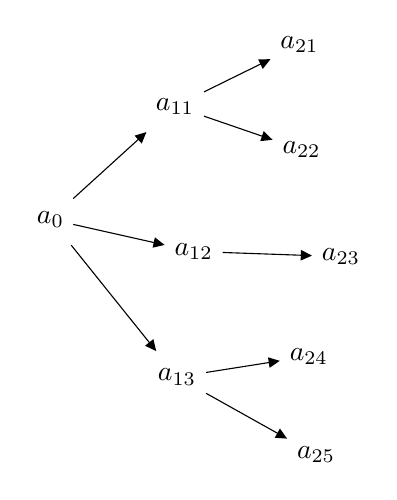
\begin{tikzpicture}[x=0.75pt,y=0.75pt,yscale=-1,xscale=1]
%uncomment if require: \path (0,300); %set diagram left start at 0, and has height of 300


% Text Node
\draw (242.02,137) node    {$a_{0}$};
% Text Node
\draw (302.02,82.5) node    {$a_{11}$};
% Text Node
\draw (311.02,152.5) node    {$a_{12}$};
% Text Node
\draw (303.02,213) node    {$a_{13}$};
% Text Node
\draw (362.02,53) node    {$a_{21}$};
% Text Node
\draw (363.02,103.5) node    {$a_{22}$};
% Text Node
\draw (382.02,155) node    {$a_{23}$};
% Text Node
\draw (366.52,203) node    {$a_{24}$};
% Text Node
\draw (370.02,250.5) node    {$a_{25}$};
% Connection
\draw    (253.02,127.01) -- (286.03,97.02) ;
\draw [shift={(288.25,95)}, rotate = 137.75] [fill={rgb, 255:red, 0; green, 0; blue, 0 }  ][line width=0.08]  [draw opacity=0] (5.36,-2.57) -- (0,0) -- (5.36,2.57) -- cycle    ;
% Connection
\draw    (253.02,139.47) -- (294.09,148.7) ;
\draw [shift={(297.02,149.36)}, rotate = 192.66] [fill={rgb, 255:red, 0; green, 0; blue, 0 }  ][line width=0.08]  [draw opacity=0] (5.36,-2.57) -- (0,0) -- (5.36,2.57) -- cycle    ;
% Connection
\draw    (252.05,149.5) -- (291.1,198.16) ;
\draw [shift={(292.98,200.5)}, rotate = 231.25] [fill={rgb, 255:red, 0; green, 0; blue, 0 }  ][line width=0.08]  [draw opacity=0] (5.36,-2.57) -- (0,0) -- (5.36,2.57) -- cycle    ;
% Connection
\draw    (316.02,75.62) -- (345.32,61.21) ;
\draw [shift={(348.02,59.88)}, rotate = 153.82] [fill={rgb, 255:red, 0; green, 0; blue, 0 }  ][line width=0.08]  [draw opacity=0] (5.36,-2.57) -- (0,0) -- (5.36,2.57) -- cycle    ;
% Connection
\draw    (316.02,87.32) -- (346.18,97.7) ;
\draw [shift={(349.02,98.68)}, rotate = 199] [fill={rgb, 255:red, 0; green, 0; blue, 0 }  ][line width=0.08]  [draw opacity=0] (5.36,-2.57) -- (0,0) -- (5.36,2.57) -- cycle    ;
% Connection
\draw    (325.02,152.99) -- (365.02,154.4) ;
\draw [shift={(368.02,154.51)}, rotate = 182.02] [fill={rgb, 255:red, 0; green, 0; blue, 0 }  ][line width=0.08]  [draw opacity=0] (5.36,-2.57) -- (0,0) -- (5.36,2.57) -- cycle    ;
% Connection
\draw    (317.02,210.8) -- (349.55,205.67) ;
\draw [shift={(352.52,205.2)}, rotate = 171.05] [fill={rgb, 255:red, 0; green, 0; blue, 0 }  ][line width=0.08]  [draw opacity=0] (5.36,-2.57) -- (0,0) -- (5.36,2.57) -- cycle    ;
% Connection
\draw    (317.02,220.84) -- (353.4,241.2) ;
\draw [shift={(356.02,242.66)}, rotate = 209.24] [fill={rgb, 255:red, 0; green, 0; blue, 0 }  ][line width=0.08]  [draw opacity=0] (5.36,-2.57) -- (0,0) -- (5.36,2.57) -- cycle    ;

\end{tikzpicture}

    % \includegraphics*[width=\textwidth]{imagefile}

    \caption{现实与可能}
    \label{现实与可能}
\end{figure}

现实与可能实际上是一对相当 “历史” 的概念。所谓现实,可以理解为是当下的
历史节点,而所谓可能,则是立足于当下,我们未来的一些发展趋势。
如图 \ref{现实与可能} 所示,如果立足于 $a_0$, 那么 $a_{11}$,
$a_{12}$ 和 $a_{13}$ 就是这个现实下的 “可能”。一旦主客观条件
成熟,历史的节点就会来到它们中的一个(也有可能是图中没有画出来的另外
的 $a_0$ 的后继节点),这是原先的 “可能” 就转化为了新的历史条件
下的 “现实”,而新的现实则产生了更多新的可能性。
事实上,图 \ref{现实与可能} 中的根节点 $a_0$ 其实也曾是更前面的
现实的可能,只不过我们在这里并没有画出来。

可能与现实的辩证统一告诉我们,尽管时间是具有一维性的,但历史的选择从来
不是只有单一选项。在面对选择的历史的十字路口的时候
(或者是面对个人自己的一些需要做出决策的问题的时候),我们需要立足现实,
展望未来,注意分析事物发展的各种可能,发挥主观能动性,做好应对不利情况
的准备,争取实现好的可能。然而遗憾的是,一个可能的好坏,往往要等到
它成为了现实之后才能明显地感觉出来,对于深处选择题中的我们,更多时候
感受到的都是茫然和无措。

区分可能与不可能的依据,是 {\kaishu 这件事在现实中是否有根据}。
区分现实的可能与抽象(潜在)的可能的依据是 {\kaishu 这件事在现实中的根据是否充分}。

\section{唯物辩证法是认识世界和改造世界的根本方法}

唯物辩证法本质上是批判的和革命的。

唯物辩证法是客观辩证法与主观辩证法的统一。具体而言:

\begin{enumerate}[label={$\left.\arabic*\right)$}, itemsep=0pt]
    \item 客观辩证法是指客观事物或客观存在的辩证法,即客观事物以相互作用、
    相互联系的形式呈现出的各种物质形态的辩证运动和发展规律。
    它存在于客观的物质世界中,可以离开人的意识、思维而独立存在,
    不以人的意志为转移。
    \item 主观辩证法
    是指人类认识和思维运动的辩证法,即以概念作为思维细胞的辩证思维运动和
    发展的规律。它存在于意识对客观物质世界的反映之中。
\end{enumerate}

这就是说,主观辩证法是意识对客观辩证法的反映。

\begin{thebibliography}{1}
    \addcontentsline{toc}{section}{参考文献}
    \bibitem{2023版教材}
    《马克思主义基本原理 (2023 版)》编写组. 马克思主义基本原理: 2023 版[M].
    北京: 高等教育出版社, 2023.
    \bibitem{核心考案}
    徐涛主编, 考研政治核心考案[M], 北京:中国政法大学出版社, 2023.1
    \bibitem{优题库}
    徐涛主编, 考研政治通关优题库[M], 北京:中国政法大学出版社, 2023.2
    \bibitem{真题库}
    徐涛主编, 考研政治必刷真题库[M], 北京:中国政法大学出版社, 2023.2
    \bibitem{冲刺背诵笔记}
    徐涛主编, 考研政治冲刺背诵笔记[M], 北京:中国政法大学出版社, 2023.9
    \bibitem{预测}
    徐涛主编, 考研政治预测 6 套卷[M], 北京:中国政法大学出版社, 2023.10
    \bibitem{预测}
    徐涛, 曲艺主编, 考研政治考前预测必备 20 题[M], 北京:中国政法大学出版社, 2023.11
\end{thebibliography}

\end{document}